% =====================================================================
%  Post-answer degeneration under EOS mismatch (no-EOS-fix OPD / TTRL)
%
%  Self-contained figure, 16.0cm x 5.8cm  ->  fits ACL \textwidth
%  (use with \includegraphics[width=\textwidth]{...} inside figure*)
%
%  Compile (two passes, `remember picture` needs the .aux):
%    pdflatex fig_no_fix_tail_examples.tex
%
%  Colour semantics
%    green      tokens up to the first correct boxed answer
%    grey       redundant post-answer suffix / elided continuation
%    pale red   the first anomalous continuation, and the repeat badge
%
%  Every number below is measured, not estimated; see
%    analysis/no_fix_tail_examples_stats.py
%  over eval_outputs/opd_ttrl_baseline_sampled_clean_bs16_n4_200step_
%       20260901_ttrl_baseline_think-false_m8192_n16_4gpu
%    (a) amc23  ex 10, seed 8,  step 100
%    (b) aime24 ex 7,  seed 1,  step 100
%    (c) amc23  ex 0,  seed 13, step 200
% =====================================================================
\documentclass[10pt]{article}
\usepackage[T1]{fontenc}
\usepackage[utf8]{inputenc}
\usepackage{tgheros}
\renewcommand{\familydefault}{\sfdefault}
\usepackage[scaled=0.86]{beramono}
\usepackage{tikz}
\usepackage[paperwidth=16.0cm,paperheight=5.8cm,margin=0pt]{geometry}
\setlength{\parindent}{0pt}
\pagestyle{empty}

% ------------------------------- palette ----------------------------
\definecolor{rowbg}{HTML}{F5F2EF}        % warm grey row band
\definecolor{cardline}{HTML}{E4DFDA}     % white code-card border
\definecolor{barbg}{HTML}{D9D5D0}        % post-answer suffix
\definecolor{barline}{HTML}{C4BFB9}
\definecolor{okgreen}{HTML}{2F7D5C}      % correct answer
\definecolor{palered}{HTML}{B85C54}      % first anomalous continuation
\definecolor{badgebg}{HTML}{F7E4E1}      % repeat badge
\definecolor{badgefg}{HTML}{A8483F}
\definecolor{ink}{HTML}{1A1A1A}
\definecolor{mid}{HTML}{4E4E53}
\definecolor{soft}{HTML}{93938F}         % elided continuation

% ---- monochrome stand-ins for the emoji the model actually emits ----
\newcommand{\iconcheck}[1]{\tikz[baseline=-0.52ex]{%
  \fill[#1,rounded corners=0.35pt] (0,-0.082) rectangle (0.212,0.122);
  \draw[white,line width=0.4pt,line cap=round,line join=round]
    (0.052,0.026)--(0.093,-0.031)--(0.166,0.070);}}
\newcommand{\iconalert}[1]{\tikz[baseline=-0.52ex]{%
  \fill[#1,rounded corners=0.35pt] (0,-0.082) rectangle (0.212,0.122);
  \fill[white] (0.093,-0.006) rectangle (0.119,0.084);
  \fill[white] (0.093,-0.052) rectangle (0.119,-0.028);}}

% ------------------------------- fonts ------------------------------
\newcommand{\panf}{\fontsize{8.0}{9.0}\selectfont\bfseries}
\newcommand{\namef}{\fontsize{7.8}{8.8}\selectfont\bfseries}
\newcommand{\smallf}{\fontsize{6.9}{8.2}\selectfont}
\newcommand{\monof}{\fontsize{6.9}{9.0}\selectfont\ttfamily}

% ------------------------------- geometry ---------------------------
\def\RX{0.06}\def\RW{15.88}       % row band
\def\PX{0.24}                     % panel letter
\def\BX{0.68}\def\BW{4.90}        % length bar
\def\EX{6.00}\def\EW{9.72}        % white code card
\def\CAP{8192}
\newcommand{\EWtext}{9.32cm}      % text width inside the code card

% #1 y0 | #2 letter | #3 name | #4 answer token | #5 pretty | #6 suffix | #7 pct
\newcommand{\Row}[7]{%
  \pgfmathsetmacro{\gw}{\BW*(#4/\CAP)}%
  \fill[rowbg,rounded corners=3pt] (\RX,#1) rectangle (\RX+\RW,#1+1.74);
  \node[anchor=base west,font=\panf,ink]  at (\PX,#1+1.40) {#2};
  \node[anchor=base west,font=\namef,ink] at (\BX,#1+1.40) {#3};
  \begin{scope}
    \clip[rounded corners=1.2pt] (\BX,#1+0.68) rectangle (\BX+\BW,#1+1.10);
    \fill[barbg]   (\BX,#1+0.68) rectangle (\BX+\BW,#1+1.10);
    \fill[okgreen] (\BX,#1+0.68) rectangle (\BX+\gw,#1+1.10);
  \end{scope}
  \draw[barline,line width=0.4pt,rounded corners=1.2pt]
       (\BX,#1+0.68) rectangle (\BX+\BW,#1+1.10);
  \node[anchor=east,mid,font=\smallf] at (\BX+\BW-0.14,#1+0.875)
       {#6 redundant tokens (#7\%)};
  \node[anchor=north west,font=\smallf,mid] at (\BX,#1+0.60)
       {first correct answer: \textcolor{okgreen}{\textbf{#5}}};
  \draw[cardline,fill=white,rounded corners=2.0pt,line width=0.45pt]
       (\EX,#1+0.16) rectangle (\EX+\EW,#1+1.58);
}
\newcommand{\Badge}[1]{\tikz[baseline=(bg.base)]{%
  \node[name=bg,fill=badgebg,rounded corners=1.6pt,inner xsep=2.8pt,inner ysep=1.4pt,
        text=badgefg,font=\normalfont\sffamily\bfseries\fontsize{6.6}{7.4}\selectfont]
       {repeated #1$\times$};}}

\begin{document}%
\begin{tikzpicture}[remember picture,overlay,x=1cm,y=1cm,inner sep=0,outer sep=0,
                    shift={(current page.south west)}]

% ================================ (a) ===============================
\def\ya{4.00}
\Row{\ya}{(a)}{Answer repetition}{1094}{1{,}094}{7{,}098}{86.6}
\node[anchor=west,align=left,font=\monof,soft] at (\EX+0.20,\ya+0.87)
 {\begin{tabular}{@{}l@{}}
   \textcolor{ink}{\#\#\# Final Answer:}\ \ \textcolor{okgreen}{\textbackslash boxed\{5\}}\\
   \textcolor{palered}{-{}-{}-\ \ \#\#\# Final Answer:\ \ \textbackslash boxed\{5\}}\\
   \makebox[\EWtext][s]{-{}-{}-\ \ \#\#\# Final Answer:\ \ \textbackslash boxed\{5\}\ \ \ldots
     \hfill\Badge{704}}
  \end{tabular}};

% ================================ (b) ===============================
\def\yb{2.03}
\Row{\yb}{(b)}{Self-correction loop}{759}{759}{7{,}433}{90.7}
\node[anchor=west,align=left,font=\monof,soft] at (\EX+0.20,\yb+0.87)
 {\begin{tabular}{@{}l@{}}
   \textcolor{ink}{\#\#\# Final Answer:}\ \ \textcolor{okgreen}{\textbackslash boxed\{25\}}\\
   \textcolor{palered}{\#\#\# Verification:\ \ Let's try x = 2, y = 12.5.\ \ Not 10.}\\
   \makebox[\EWtext][s]{Let's try x = 2, y = 12.5.\ \ \ldots\hfill\Badge{368}}
  \end{tabular}};

% ================================ (c) ===============================
\def\yc{0.06}
\Row{\yc}{(c)}{Token repetition}{462}{462}{7{,}730}{94.4}
\node[anchor=west,align=left,font=\monof,soft] at (\EX+0.20,\yc+0.87)
 {\begin{tabular}{@{}l@{}}
   \textcolor{ink}{\#\#\# Final Answer:}\ \ \textcolor{okgreen}{\textbackslash boxed\{27\}}\\
   \textcolor{palered}{They meet **27 miles from City A**.}\ \iconalert{palered}\,%
     \iconalert{palered}\,\iconalert{palered}\,\iconcheck{palered}\,\iconcheck{palered}\,%
     \iconcheck{palered}\,\iconcheck{palered}\,\iconcheck{palered}\\
   \makebox[\EWtext][s]{\iconcheck{soft}\,\iconcheck{soft}\,\iconcheck{soft}\,%
     \iconcheck{soft}\,\iconcheck{soft}\,\iconcheck{soft}\,\iconcheck{soft}\,%
     \iconcheck{soft}\,\iconcheck{soft}\ \ldots\hfill\Badge{3{,}836}}
  \end{tabular}};
\end{tikzpicture}
\end{document}
